\subsection{Anti-Aliasing Filter} \label{subsec:AAFilter}

An anti-aliasing filter is added before the ADC inputs to prevent aliasing effects. A number of considerations were made for this filter regarding the desired frequency response and order of the filter. These consideration can be seen in appendix \refq{App:AntiAliasingFilterConsideration}.

Based on the findings in appendix \refq{App:AntiAliasingFilterConsideration}, the anti-aliasing filter will be a 4th order butterworth low-pass filter to ensure maximum passband flatness and to have a minimum amount of attenuation at \SIQ{1}{\mega\hertz}, which is the highest test signal frequency that the ADC can expect to sample. Furthermore, the filter should have a gain of \SIQ{0}{\decibel} in the passband, so the filter must also be an active filter design, as the one shown on figure \refq{fig_7_1_4_SALLENKEY}.

\begin{figure}[H]
    \centering
    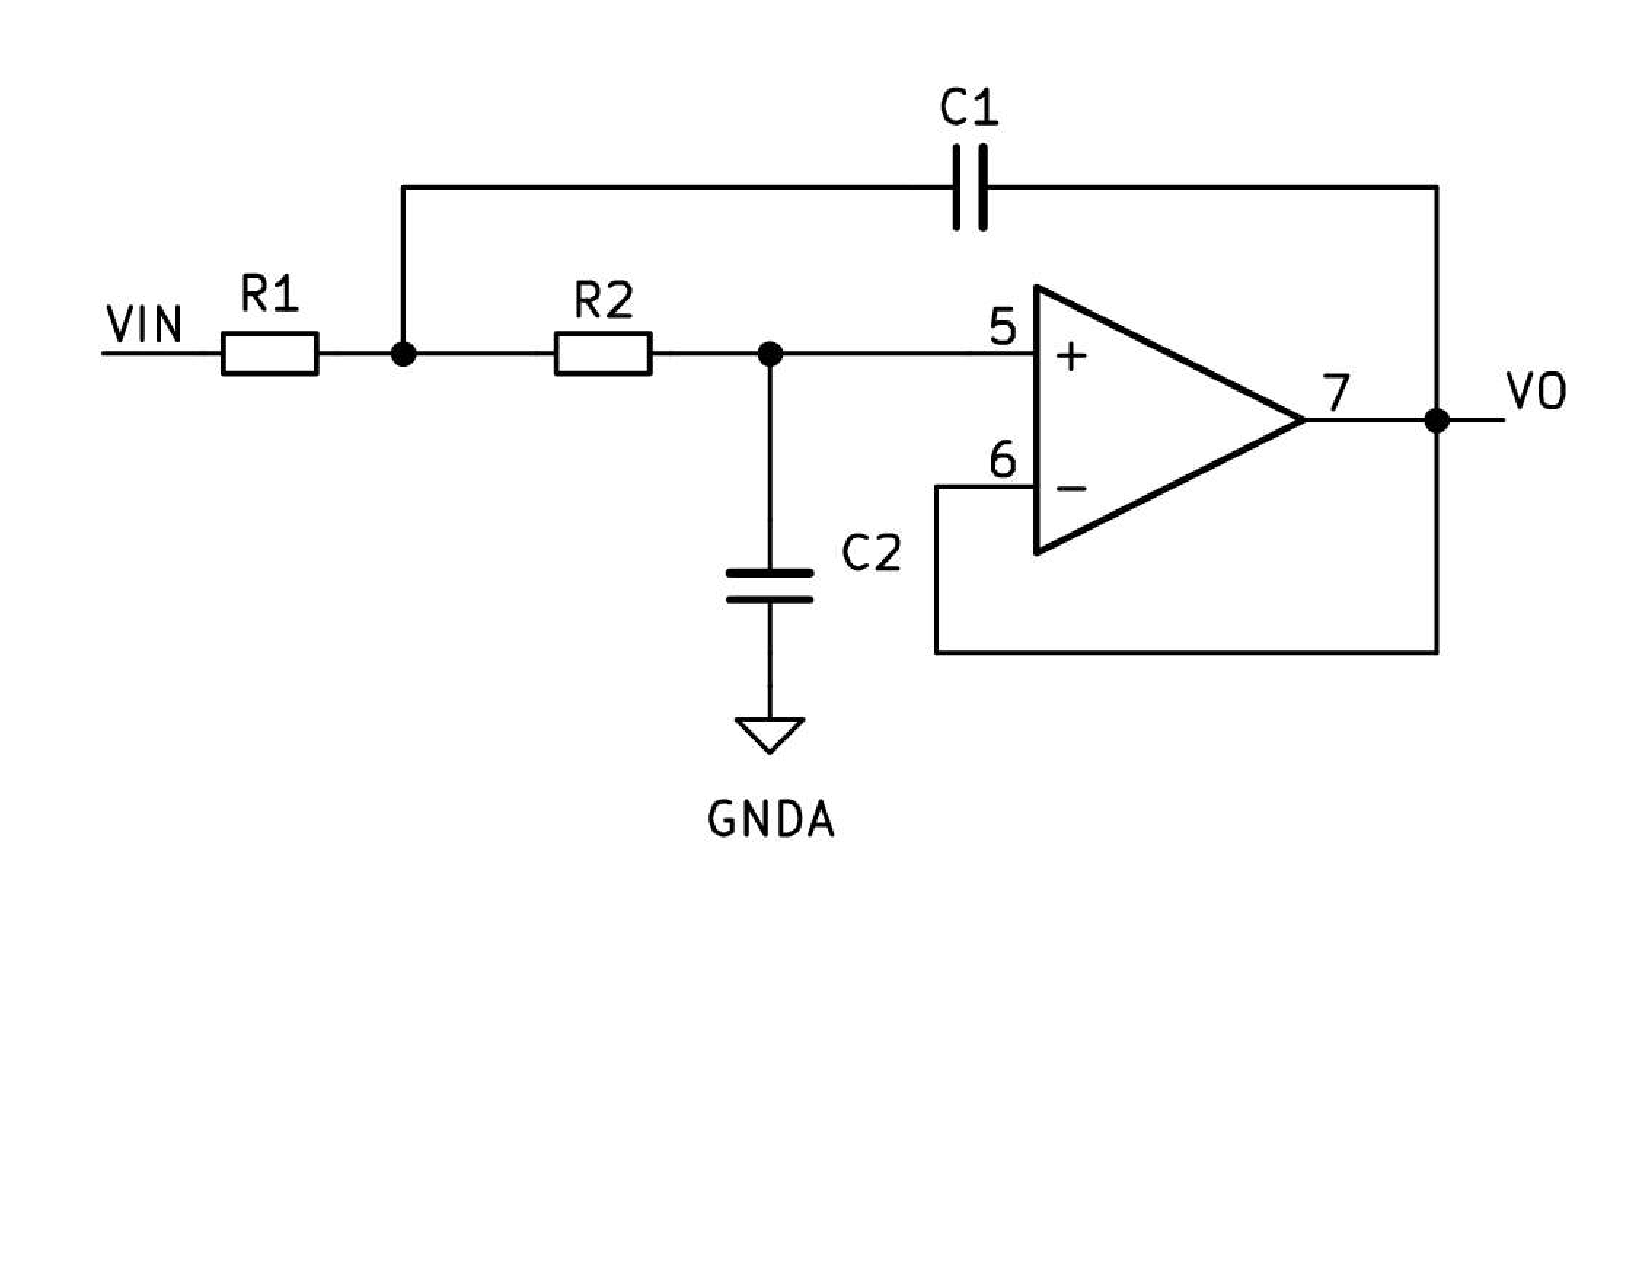
\includegraphics[clip, trim=0 150 0 0, width=0.6\textwidth]{Sections/7_SystemDesign/Figures/7_1_4_AAF_SALLENKEY.pdf}
    \caption{A Sallen-Key lowpass filter prototype.}
    \label{fig_7_1_4_SALLENKEY}
\end{figure}

To make the filter we first find the poles with eq \refq{eq:7_1_4_LPPoles}\cite{ANALOGFILTERS}.
\begin{equation}\label{eq:7_1_4_LPPoles}
    P_k = e^{j(\frac{2k-1}{2n}\pi + \frac{\pi}{2}  )} 
\end{equation}
Where $n = 4$ is the order of the filker and $k = 1..n$. This will give two complex conjugated pair of poles as seen in equation xyz

\begin{equation}\label{eq:7_1_4_LPPoles1} 
    \begin{aligned}
        P_1 &= e^{j\left(\frac{2-1}{6}\pi + \frac{\pi}{2}\right)} = e^{\frac{j5}{8}\pi} \approx -0.3827 + j0.9239 \\
        P_2 &= e^{j\left(\frac{4-1}{6}\pi + \frac{\pi}{2}\right)} = e^{\frac{j7}{8}\pi} \approx -0.9239 + j0.3827 \\
        P_3 &= e^{j\left(\frac{6-1}{6}\pi + \frac{\pi}{2}\right)} = -e^{\frac{j}{8}\pi} \approx -0.9239 - j0.3827  \\
        P_3 &= e^{j\left(\frac{8-1}{6}\pi + \frac{\pi}{2}\right)} = -e^{\frac{j3}{8}\pi}\approx -0.3827 - j0.9239 
    \end{aligned}
\end{equation}

The poles will be used to form two second order systems, so the conjugated pole pairs are grouped up. $P_1$ and $P_4$ is a conjugated pair and so is $P_2$ and $P_3$. The poles are frequency scaled to produce the desired response. As the design goal is to have $f_{-3db} = 1e6$ then this will be used as the frequency scaling factor as shown in eq \ref{eq:7_1_4_LPKF}

\begin{equation}\label{eq:7_1_4_LPKF}
    k_f = \omega_{f3db} = 2\pi 2E6 = 1.2567E7
\end{equation}

The scaled poles will form the transferfunction in equation \refq{eq:7_1_4_LPTF}.
\begin{equation}\label{eq:7_1_4_LPTF}
    \begin{aligned}
    H_{LP}(s) = \frac{1}{(s-P_1\cdot k_f)(s-P_4\cdot k_f)  }\cdot \frac{1}{(s-P_2\cdot k_f)(s-P_3\cdot k_f)}\\
    H_{LP}(s) = \frac{1}{s^2 + 9.617E6s + 1.5791E14}\cdot \frac{1}{s^2 + 2.3220E7s + 1.5791E14}
\end{aligned}
\end{equation}

The frequency scaling factor has been multiplied 4 times in the denominator and has to be added to the numerator to set the correct gain, or natural frequency. This can be seen in eq \refq{eq:7_1_4_LPTFKFSQ}
\begin{equation}\label{eq:7_1_4_LPTFKFSQ}
    \begin{aligned}
        H_{LP}(s) = \frac{k_f^2}{s^2 + 9.617E6s + 1.5791E14}\cdot \frac{k_f^2}{s^2 + 2.3220E7s + 1.5791E14}\\
    H_{LP}(s) = \frac{1.5791E14}{s^2 + 9.617E6s + 1.5791E14}\cdot \frac{1.5791E14}{s^2 + 2.3220E7s + 1.5791E14}
\end{aligned}
\end{equation}

The transferfunction for the low-pass filter is plotted to see the magnitude response, the results can be seen on figure \refq{fig_7_1_4_MAGRESP}.
\begin{figure}[H]
    \centering
    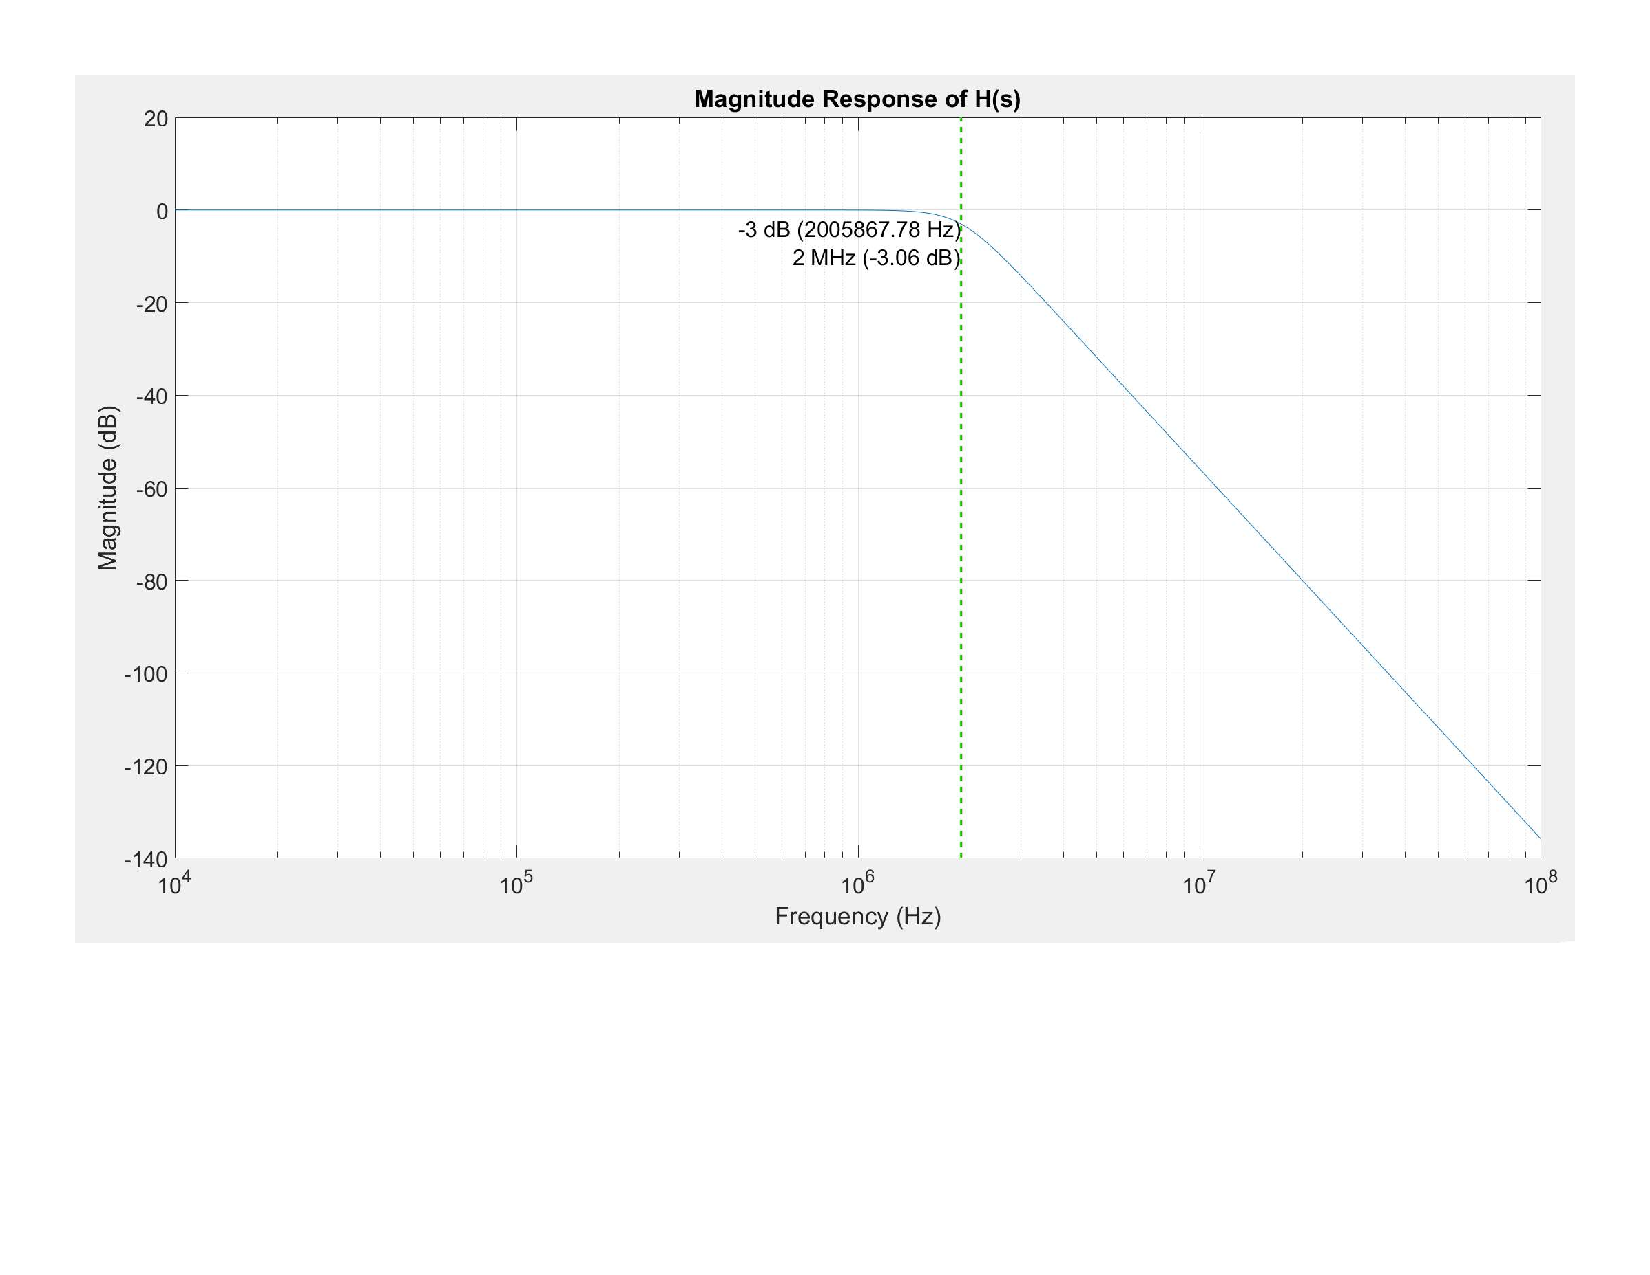
\includegraphics[clip, trim=0 150 0 0, width=1\textwidth]{Sections/7_SystemDesign/Figures/7_2_4_AAFILT_HS.pdf}
    \caption{The magnitude response for the low-pass filter.}
    \label{fig_7_1_4_MAGRESP}
\end{figure}

The filter will be made by cascading two Sallen-Key second-order biquads to form a 4th order filter. The network function for a Sallen-Key biquad can be seen in equatio \refq{eq:7_1_4_SallenKeyTF} \cite{ANALOGFILTERS}.

\begin{equation}\label{eq:7_1_4_SallenKeyTF}
    V_{SK} = \frac{  \frac{\mu}{R_1R_2C_1C_2}}{s^2 + (\frac{1}{R_1C_1} + \frac{1}{R_2C_1} + \frac{1 - \mu}{R_2C_2})s + \frac{1}{R_1R_2C_1C_2}}
\end{equation}

Where $\mu$ is the gain of the OP Amp. Equation \refq{eq:7_1_4_SallenKeyTF} is a second order system of the standard form shown in eq \refq{eq:7_1_4_SecondOrderSystem}.

\begin{equation}\label{eq:7_1_4_SecondOrderSystem}
   H(s) = \frac{G\omega_0^2}{s^2 + \frac{\omega_0}{Q}s + \omega_0^2}
\end{equation}

By comparing eq \refq{eq:7_1_4_SecondOrderSystem} and eq \refq{eq:7_1_4_SecondOrderSystemQ} it is evident that the natural frequency, $\omega_0$ and the quality factor, Q, is the following.

\begin{equation}\label{eq:7_1_4_SecondOrderSystemQ}
    Q = \frac{ \frac{1}{\sqrt{R_1R_2C_1C_2}} }{ \frac{1}{R_1C_1} + \frac{1}{R_2C_1} + \frac{1-\mu}{R_2C_2}}
 \end{equation}
 \begin{equation}\label{eq:7_1_4_SecondOrderSystemNatural}
    \omega_0 = \frac{1}{\sqrt{R_1 R_2 C_1 C_2}}
 \end{equation}

 The anti-aliasing filter should have unity gain, so, $\mu = 1$. Unity gain in a Sallen-Key topology will also give the least sensitive design as the gain of the circuit is not dependant on any external resistors. For this design the resistors will be equal, so $R_1 = R_2 = R$. $R$ is arbitrarily chosen to be $R = 1e3$ and the quality factor and natural frequency will reduce to equation xyz
 \begin{equation}\label{eq:7_1_4_SecondOrderSystemQ}
    \begin{aligned}
        Q = \frac{ \frac{1}{\sqrt{C_1C_2}} }{ \frac{2}{C_1} + \frac{1-\mu}{C_2}}\\
        \omega_0 = \frac{1}{R\sqrt{C_1 C_2}}
    \end{aligned}
 \end{equation}

By comparing eq \refq{eq:7_1_4_SecondOrderSystem} and \refq{eq:7_1_4_LPTFKFSQ} it can be seen that for both second order systems the natural frequency will be eq \refq{eq:7_1_4_SecondOrderSystemNaturalFrq}.
\begin{equation}\label{eq:7_1_4_SecondOrderSystemNaturalFrq}
    \omega_0 = \sqrt{1.5791E14}
 \end{equation}

 Capacitors $C_1$ and $C_2$ can now be calculated for the first biquad. The quality factor of the biquad is found by comparing \refq{eq:7_1_4_SecondOrderSystem} to \refq{eq:7_1_4_LPTFKFSQ} and solving for Q as shown in eq \refq{eq:7_1_4_Q1}.

 \begin{equation}\label{eq:7_1_4_Q1}
    \begin{aligned}
        \frac{\sqrt{\omega_0}}{Q_1} = \frac{\sqrt{1.5791E14}}{Q_1}= 9.618\\
        Q_1 = 1.307
    \end{aligned}
 \end{equation}

 An expression is found for $C_1$ by using eq \refq{eq:7_1_4_SecondOrderSystemQ} and \refq{eq:7_1_4_Q1} as shown in equation \refq{eq:7_1_4_C1}.

 \begin{equation}\label{eq:7_1_4_C1}
    \begin{aligned}
        Q_1 = \frac{ \frac{1}{\sqrt{C_1C_2}} }{ \frac{2}{C_1} + \frac{1-\mu}{C_2}}\\
        1.307 = \frac{ \frac{1}{\sqrt{C_1C_2}} }{ \frac{2}{C_1} + \frac{1-\mu}{C_2}}\\
        C_1 = 6.829C_2
    \end{aligned}
 \end{equation}

 The expression for $C_1$ is used to find $C_2$ by using eq \refq{eq:7_1_4_SecondOrderSystemNatural} as shown in eq \refq{eq:7_1_4_C2}.
 \begin{equation}\label{eq:7_1_4_C2}
    \begin{aligned}
        \omega_0 = \frac{1}{R\sqrt{C_1C_2}}\\
        1.5791E14 = \frac{1}{1E3\sqrt{(6.829C_2)C_2}}\\
        C_2 = 3.045E-11
    \end{aligned}
 \end{equation}
 A value for $C_2$ has been found. This value is substituted into eq \refq{eq:7_1_4_C1} to find $C_1$ as shown in eq \refq{eq:7_1_4_C1_CAL}.
 \begin{equation}\label{eq:7_1_4_C1_CAL}
    \begin{aligned}
        C_1 = 6.829C_2\\
        C_1 = 6.829\cdot  3.045E-11\\
        C_2 = 2.079E-10
    \end{aligned}
 \end{equation}

 All the components for the first biquad has been established. The exact same procedure can be followed to find the components for the second biquad, by using the $\frac{\omega_0}{Q_2} = 2.3220E7$ term from the other denominator in the transferfunction in eq \refq{eq:7_1_4_LPTFKFSQ}. Using this approach the capacitors for the second biquad are $C_3 = 8.61E-11$ and $C_4 = 7.63E-11$. The final circuit for the anti-aliasing filters for one of the differential DUT signals going to the ADCs can be seen on figure \refq{fig_7_1_4_AAFILTVDUT}.

 \begin{figure}[H]
    \centering
    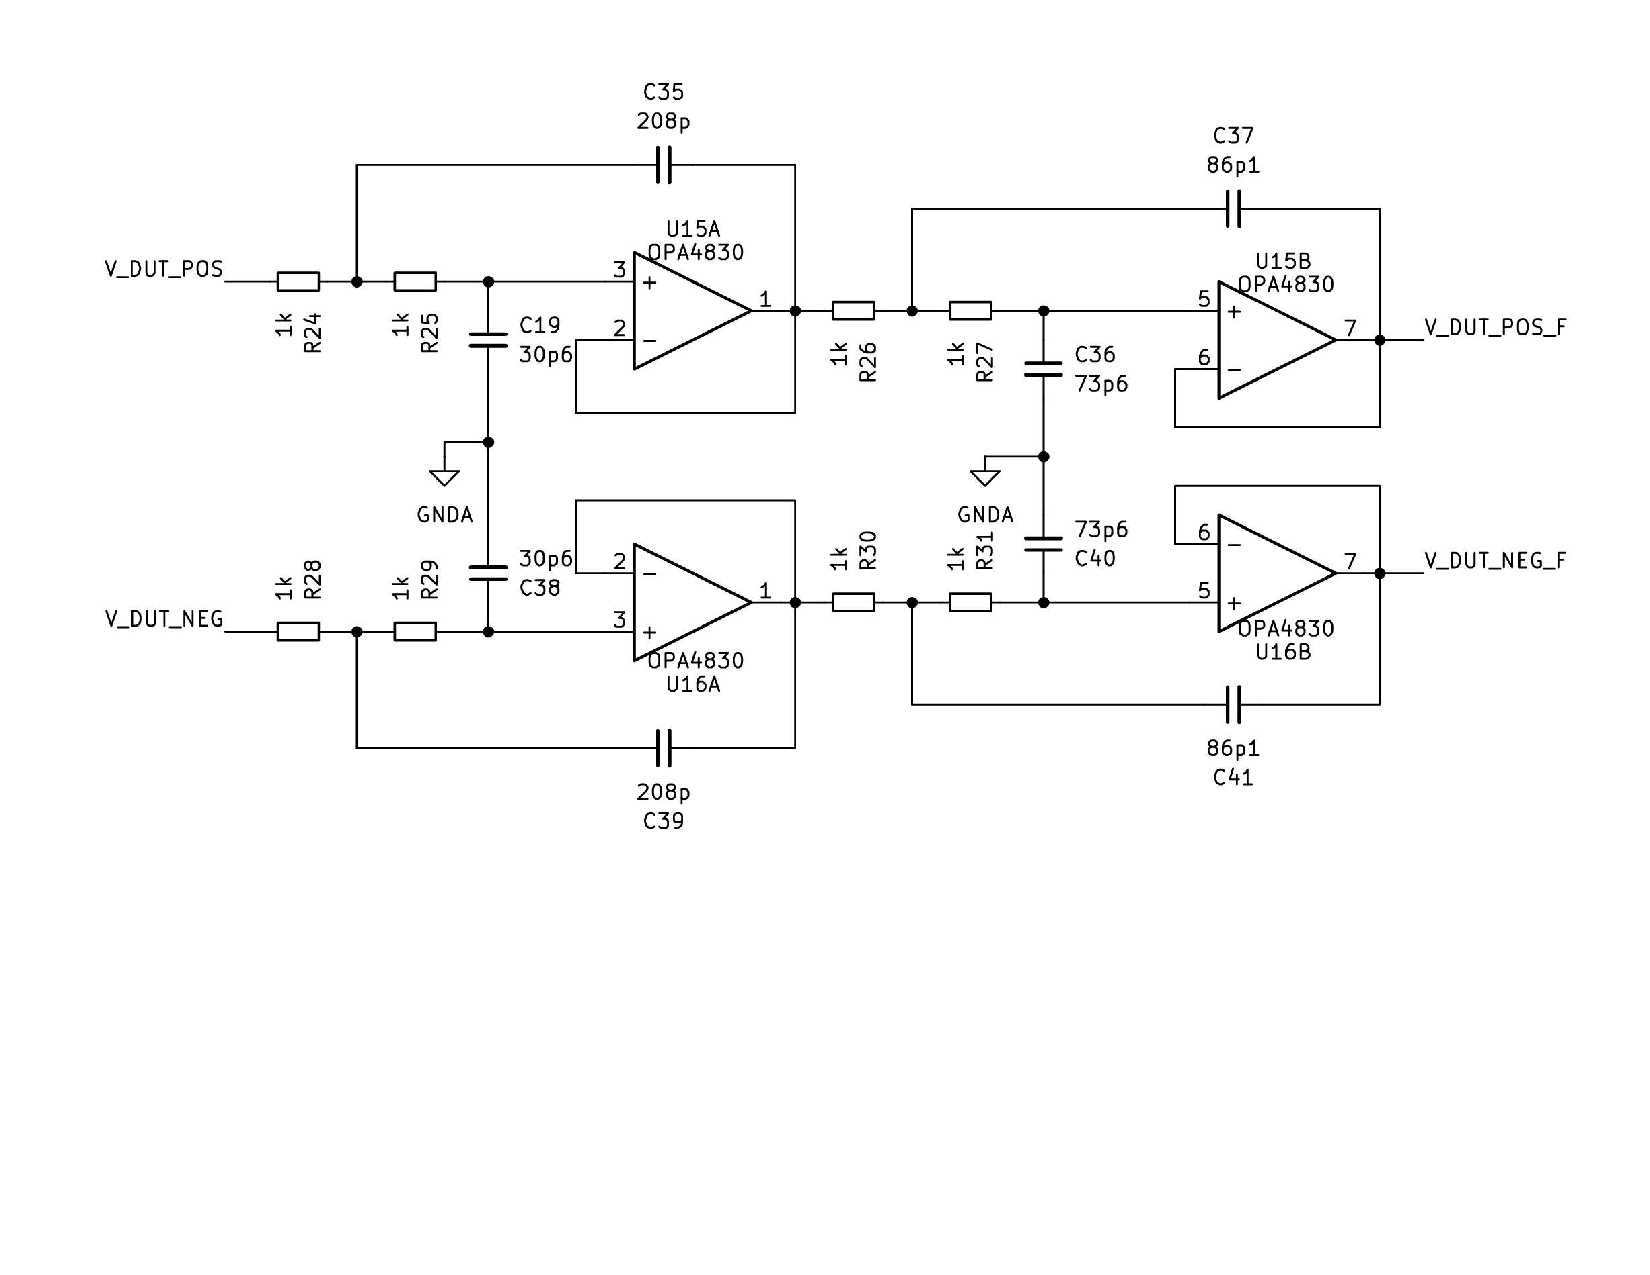
\includegraphics[clip, trim=0 200 0 0, width=1\textwidth]{Sections/7_SystemDesign/Figures/7_1_4_AAFilterSch.pdf}
    \caption{One of the anti-aliasing filters in the Analog Front End. This filter is in the signal path for the DUT voltage waveform. The current waveform will have a matching anti-aliasing filter.}
    \label{fig_7_1_4_AAFILTVDUT}
\end{figure}

